% !TeX root = ../thuthesis-example.tex

\chapter{经典故障场景分析}\label{chap-failure-scenarios}

本章针对系统常见的故障场景,如磁盘写满、系统宕机、网络分区、集群变更等,分析了本文中提出的高可用和容错方案的支持。对于每一种故障场景,本章节都给出了错误的检测方法和容错恢复的方法。


\section{单节点磁盘写满}

单节点磁盘写满的故障指,在DataNode运行过程中,该节点可用存储空间已经完全耗尽,无法再写入任何新的数据。

\subsection{检测方法}

目前IoTDB集群中有两种单节点磁盘写满的故障检测方式。

第一种是定期预防式的诊断,通过ConfigNode和DataNode的心跳完成。ConfigNode和DataNode交换的心跳包中会带有该DataNode节点的磁盘最大容量和目前的使用情况。如果目前的使用率已经超过了预先设置的阈值,那么ConfigNode就会将该节点标志为只读的状态,标志着ConfigNode检测到了单节点磁盘写满的故障。

第二种是发生时的临诊,通过DataNode在写入过程中的自我检测来完成。在DataNode服务某一个写入请求,在文件系统上真正写入数据之前,会进行可写入性的检查。如果发现此时磁盘空间不足,那么本次写入请求就不会执行,并且返回给Session本次节点只读的状态。

\subsection{高可用容错方案}

\begin{figure}
    \centering
    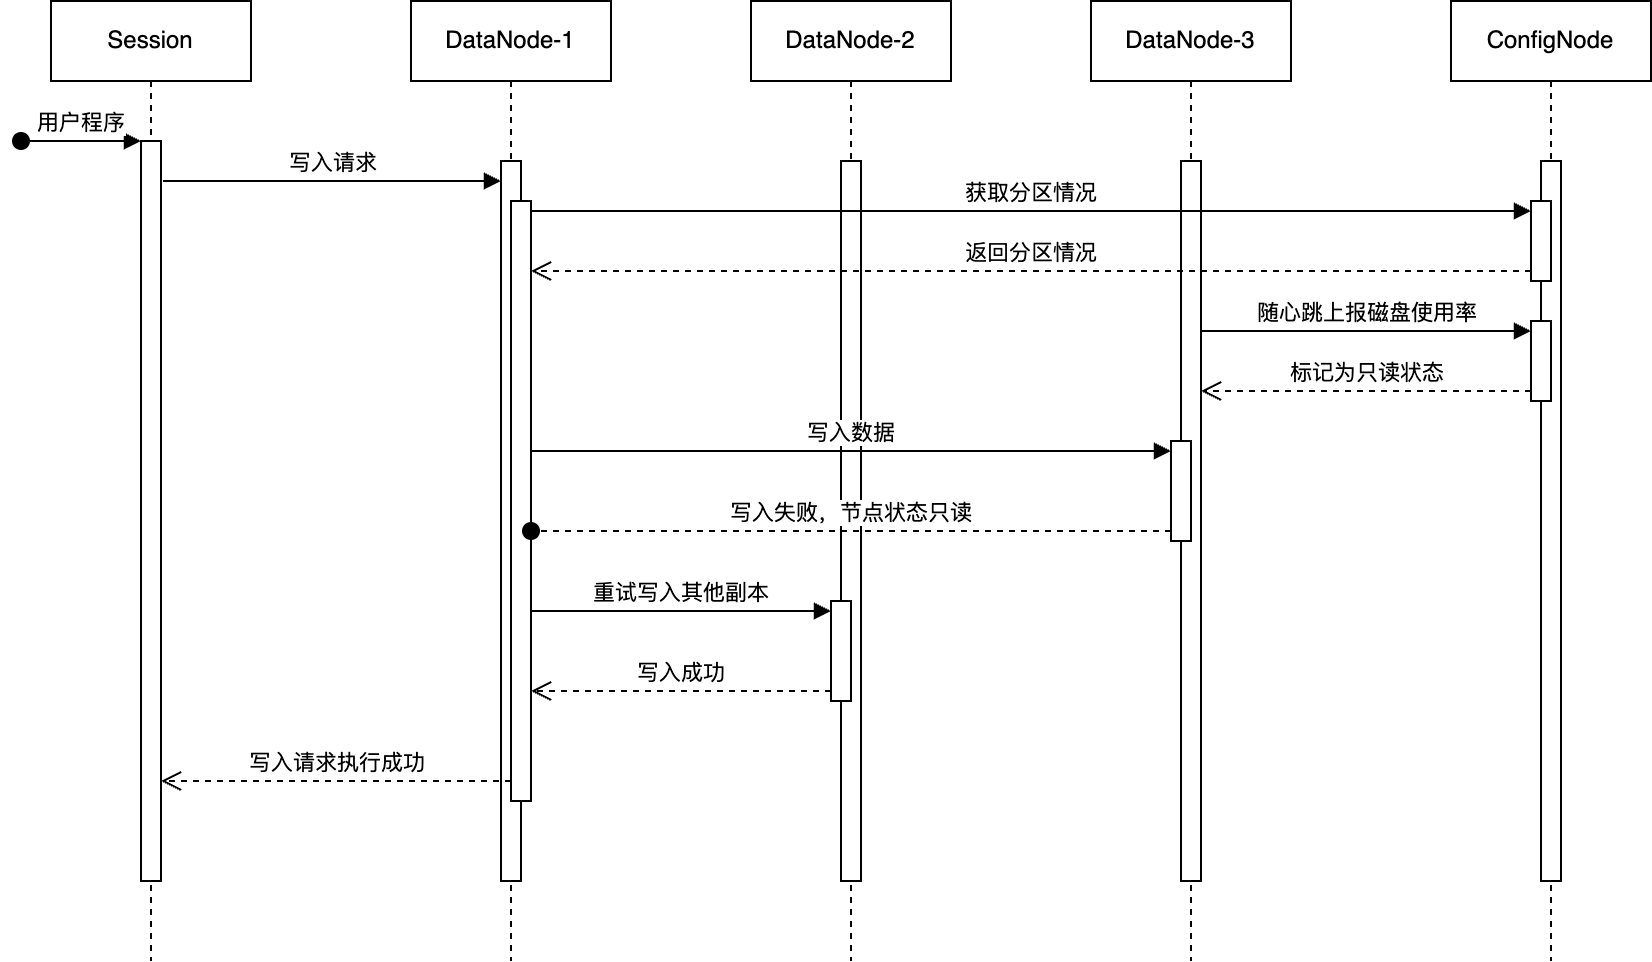
\includegraphics[width=0.99\linewidth]{c05-diskfull.png}
    \caption{单节点磁盘写满的高可用容错时序图}
    \label{fig:c05-diskfull}
  \end{figure}

图\ref{fig:c05-diskfull}给出了单节点磁盘写满的完整容错时序图。

可以看到,在某一个时刻,DataNode3的磁盘使用情况超过了阈值,并且在下一次和ConfigNode上报心跳的时候将这一情况上报给了ConfigNode。ConfigNode会将该节点标记为ReadOnly,这个信息会被同步到所有节点的协调者模块。

对于读请求来说,无论是故障发生时的在途请求,还是故障发生之后的新请求,都能够正常执行,不受任何影响。对于写请求来说,则通过前一章节描述的故障错误转移的方式来实现容错。

对于磁盘写满故障发生之后的写入请求,由协调者阶段在规划阶段进行容错处理。
在写入的规划阶段,规划器能够从ConfigNode获取最新的分区情况,明确了解该节点只读的状态,并会将本次的请求给路由到其他可以写入的副本上,从而完成写入请求的正常执行。

对于磁盘写满故障发生时就在执行的在途写入请求,通过协调者的调度阶段重试来实现容错。以图中的写入请求来说,请求在第一次规划时,DataNode3并未出现磁盘写满的故障,因此规划的结果是向这个DataNode3节点写入数据。
然而,在数据实际写入之前,DataNode3的状态变更为只读,无法服务这次的写入请求,因此本次的写入操作会返回异常。
DataNode1的协调者节点会捕捉到这次失败的调度,开启重试恢复。重试时,协调者会选择其他的可用副本所在节点(在本次请求中为DataNode2)尝试写入。由于DataNode2的状态健康,因此本次数据会写入正常运行的DataNode2中,最后实现数据的成功写入。


\section{进程宕机}

进程宕机的故障指,正在运行的DataNode进程由于内存溢出、强制终止等问题意外终止或停止响应。

\subsection{检测方法}

IoTDB通过捕捉ConfigNode和DataNode之间维持的心跳信道断开这一事件,判断DataNode的进程宕机这一故障。

如章节\ref{sec:detection-thrift}所述,ConfigNode Leader和DataNode之间的心跳通道是基于Thrift构建的,底层传输方式为Thrift的TSocket,这是一种基于TCP连接的传输。
当进程终止时,操作系统会立即关闭该进程打开的所有TCP连接。

ConfigNode Leader和DataNode之间建立的Thrift通道会因为进程宕机而断开,这一事件会被报告给ConfigNode Leader,从而使ConfigNode感知到节点宕机的故障。即使TCP连接没有立即断开,如果对端进程已经停止响应,任何尝试通过该连接进行读写操作都会导致I/O异常。Thrift框架也能够捕获这些I/O异常,例如连接超时、连接拒绝等,从而判断对端进程已失效。


\subsection{高可用容错方案}

在进程宕机的故障情况下,Session会通过自动服务发现和转移的方式将客户端的请求流量引导到新的节点上,而协调者节点会通过调度时期的容错机制将内部的碎片实例引导到其他存活节点上的副本。

\begin{figure}
    \centering
    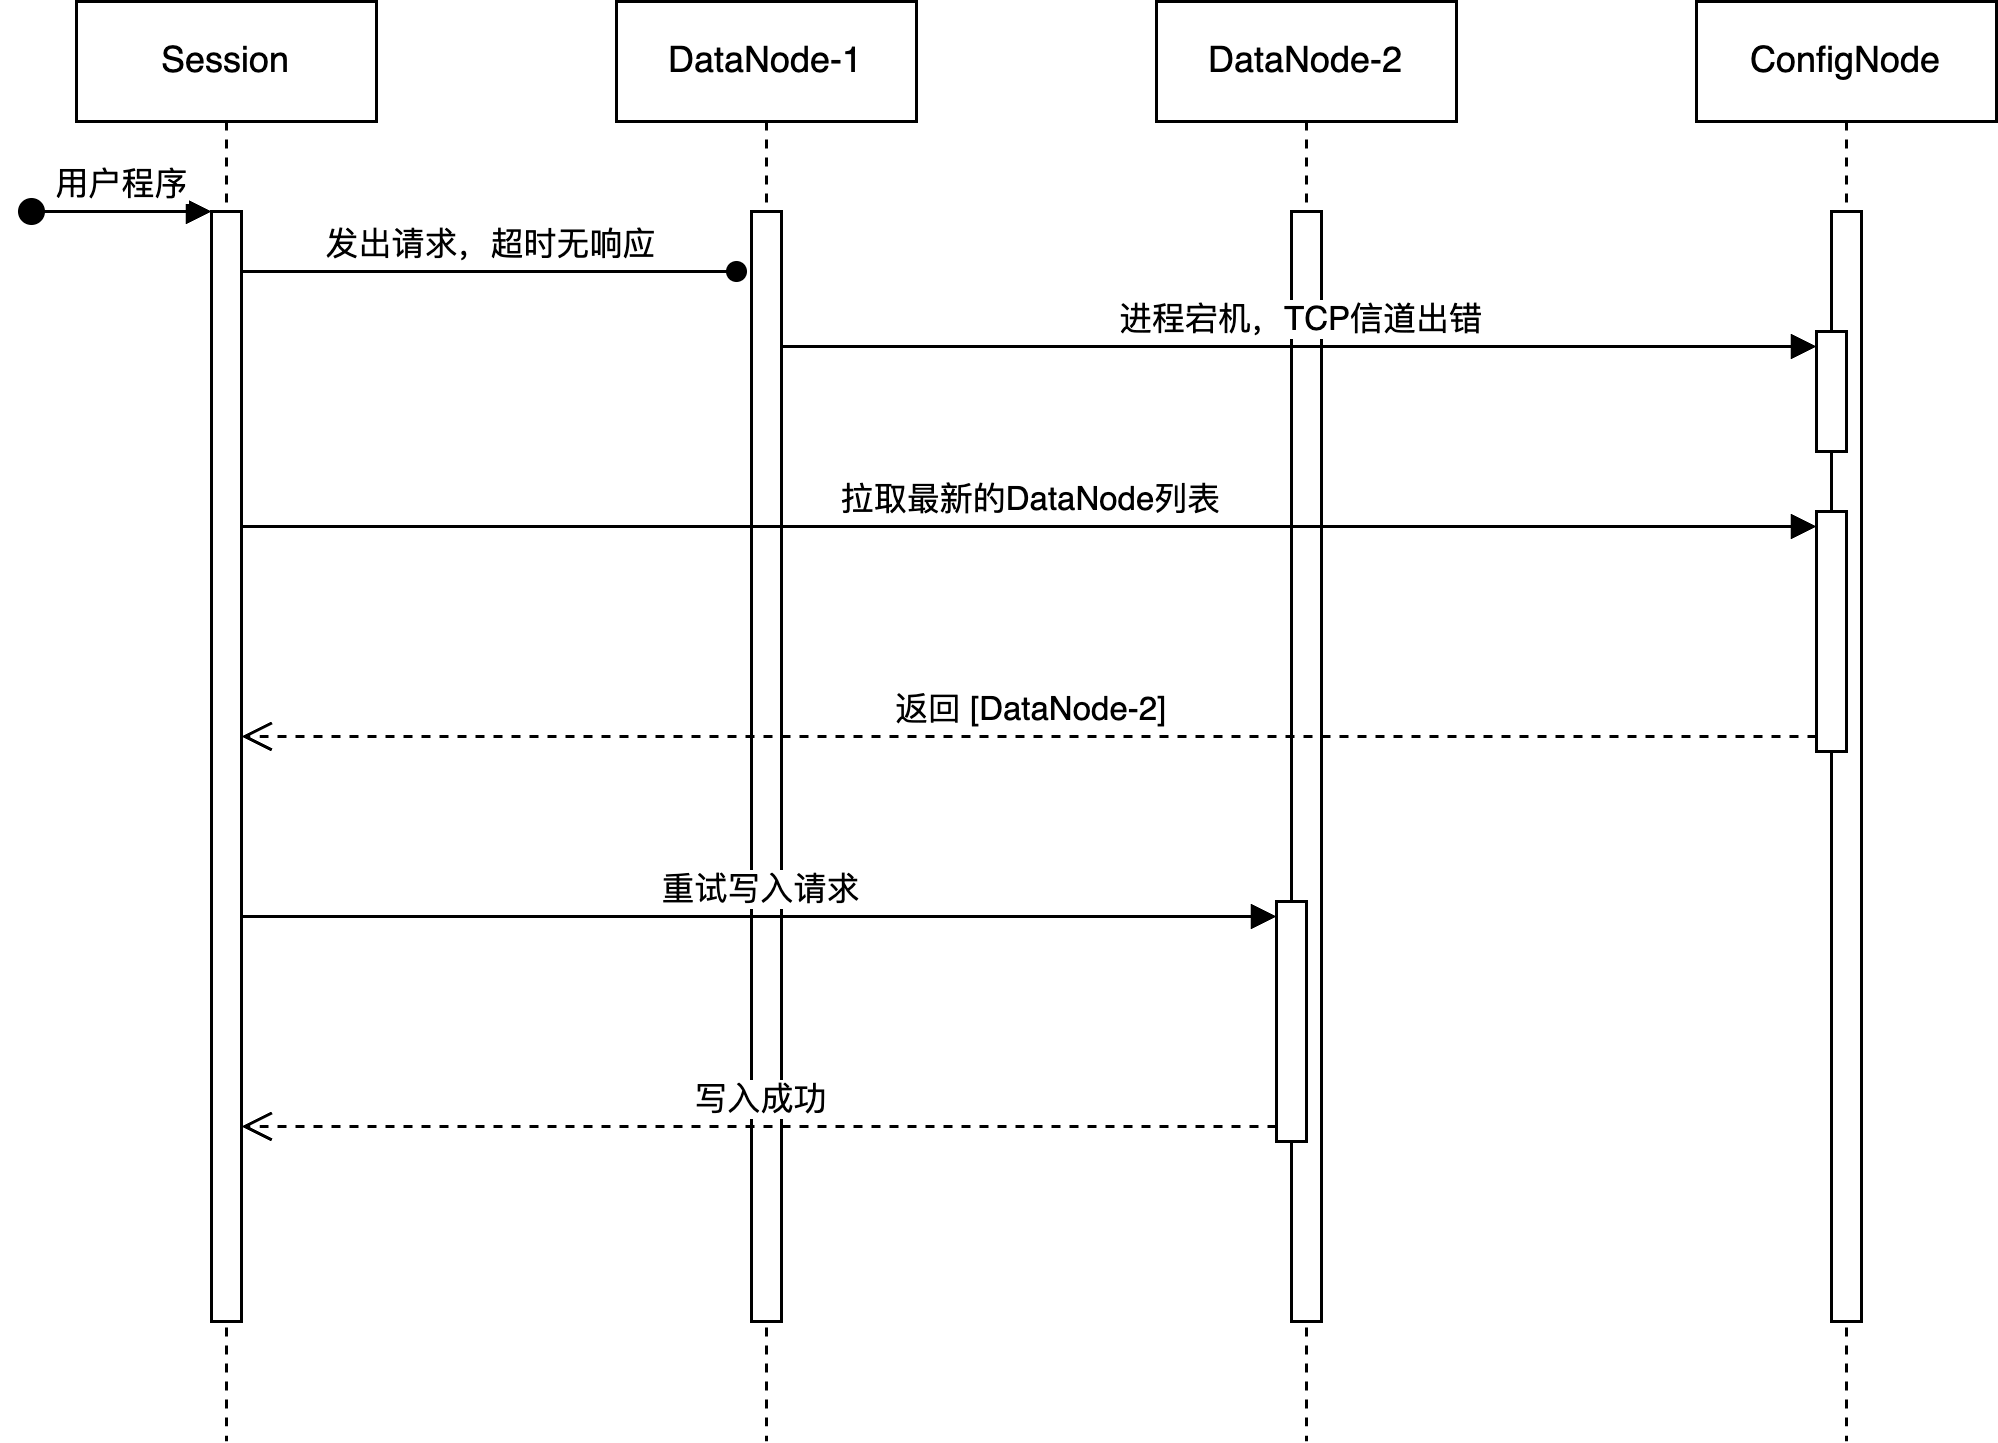
\includegraphics[width=0.99\linewidth]{c05-process-down-1.png}
    \caption{单节点进程宕机的高可用容错时序图}
    \label{fig:c05-process-down-1}
\end{figure}

图\ref{fig:c05-process-down-1}展示了Session自动服务发现和转移的容错方案。图中DataNode1在处理Session的请求的时候出现了宕机,会导致Session的该请求超时无响应。

一方面,ConfigNode通过Thrift信道的连接断开事件检测到DataNode1节点的进程异常,并会更新这个节点的状态。由于Session的后台进程会持续地从ConfigNode拉取最新的DataNode列表,因此在下一次拉取的时候,Session就能够发现DataNode1失效的问题。

另一方面,Session会尝试向其他的DataNode进行请求重试,在本例中会将请求数据引导到DataNode2上。由于此时DataNode2正常工作,因此本次请求能够被正常处理,从而使用户的请求最终能够正常写入。


对于集群内部的请求流量,例如其他节点的协调者模块发送到本DataNode1上的碎片实例,会由其他节点的协调者重试其他的数据副本,重试的算法和前一章节磁盘写满的流程图\ref{fig:c05-diskfull}相似。

\section{对称网络分区}

网络分区是指由于网络故障导致系统中的节点被分割成两个或多个相互隔离的分区。在同一个分区内的节点可以互相通信,但不同分区之间的节点无法互相通信或通信严重受阻。

对称网络分区故障是指其中一个分区无法连接任何其他分区的节点。例如,在由三个节点DataNode1、DataNode2、DataNode3组成的集群中,当DataNode1与DataNode2和DataNode3发生对称网络分区的故障,那么DataNode2和DataNode3之间的通信能够继续保持,但是两个节点都无法和DataNode1进行通信。

\subsection{检测方法}

IoTDB通过依赖ConfigNode和DataNode之间交换心跳包,根据心跳历史和Phi Accrual研判算法来检测对称网络分区。

当节点发生对称网络分区的时候,由于节点依旧存活,操作系统不会关闭TCP信道,因此我们需要依赖心跳历史的采样进行研判。由于ConfigNode将会无法和DataNode之间交换心跳,在超过一定的时间之后,Phi Accrual算法就会研判该DataNode不可达,ConfigNode Leader将会将该节点的状态设置成不可知。


\subsection{高可用容错方案}

对于发生非对称网络分区的DataNode,在事实意义上可以认为这个节点完全不可用。因此,在容错方案上,可以借鉴上一小节进程宕机的处理方法。

对于连接在该节点上的Session,可以通过\ref{fig:c05-process-down-1}所示的流程将请求流量引导到其他不分区的DataNode上。

对于协调者内部的碎片实例,可以通过\ref{fig:c05-diskfull}所示的流程将请求流量引导到其他非分区存活副本所在的DataNode上。


\section{非对称网络分区}

非对称网络分区故障可以参考图\ref{fig:c03-partition}所示。节点之间部分的网络拓扑不可达,但是没有任何一个节点无法和所有的其他节点都无法通信。

\subsection{检测方法}

IoTDB通过DataNode之间的对等心跳来检测非对称网络分区的故障。在非对称网络分区的情况下,由于所有的DataNode依然能够和ConfigNode之间正常交换心跳包,因此无论是通过Thrift心跳通道,还是通过ConfigNode的心跳和研判算法都无法检测出非对称网络分区的故障。

此时,需要通过章节\ref{sec:datanode-intra-heartbeat}所述的DataNode之间的对等心跳来检测。
DataNode之间会定期和所有的其他DataNode之间交换心跳,验证连通性。如果DataNode1和DataNode2发生了非对称网络分区,那么DataNode1和DataNode2之间无法进行心跳交换。DataNode1和DataNode2分别会将这个情况上报给ConfigNode Leader。ConfigNode Leader会通过Phi Accrual算法分析对等心跳,并且研判出DataNode1和DataNode2之间出现了非对称网络分区的问题,实现故障的检测。


\subsection{容错方案}

IoTDB通过协调者在规划阶段的容错和Session侧的协同来共同解决非对称网络分区的问题。

\begin{figure}
    \centering
    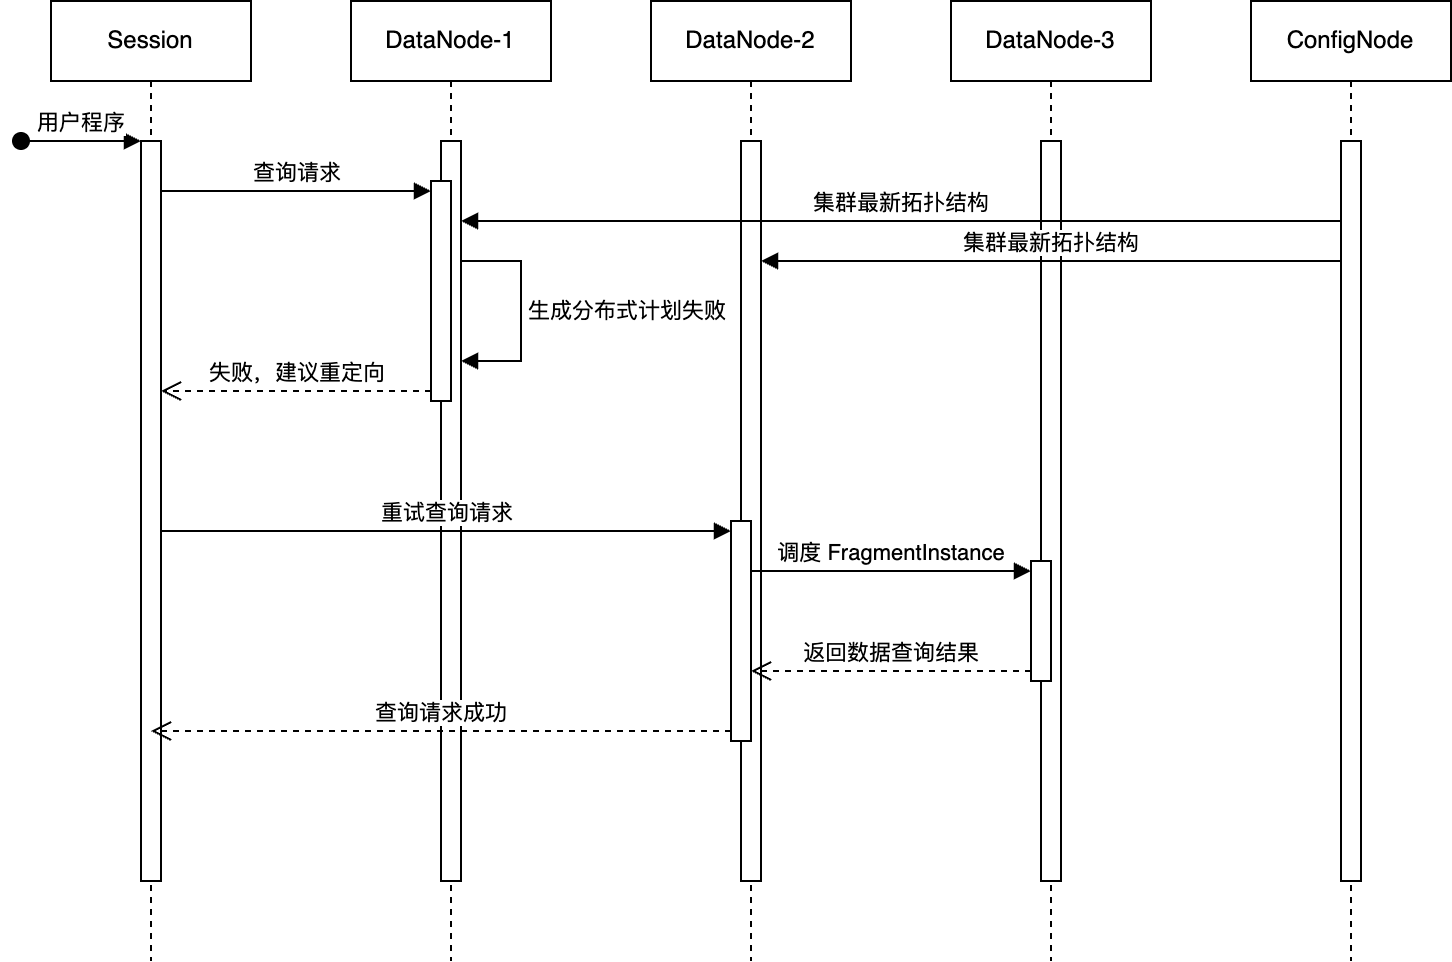
\includegraphics[width=0.99\linewidth]{c05-partition-asym.png}
    \caption{非对称网络分区的高可用容错时序图}
    \label{fig:c05-partition-asym}
\end{figure}

图\ref{fig:c05-partition-asym}给出了非对称网络分区的高可用容错时序图。假设集群DataNode1和DataNode3之间出现了非对称网络分区。当Session连接到DataNode1上并发送了查询请求,在DataNode1上的协调者会解析规划这个查询请求。假设这次查询请求的碎片实例将会被调度到所有的DataNode1、DataNode2、DataNode3上,此时根节点的碎片实例必须被调度到能同时和三个节点的联通的DataNode,即DataNode2上。因此,本次规划会立即失败,向Session返回失败的状态码,并建议Session将请求重定向到DataNode上执行。

Session在遇到失败的状态码的时候,会重新将请求定向到DataNode2上执行。由于DataNode2并不存在网络分区的问题,能够与集群内的所有节点正常连接,因此查询规划能够顺利生成和调度,在三个DataNode之间进行数据的实际查询和数据聚合,完成本次的查询请求,将结果返回给Session的客户端。

\section{ConfigNode节点脑裂}

脑裂是IoTDB系统中面临的一个严重业务问题。

ConfigNode是集群的大脑,负责管理集群的节点基础信息、当前状态、集群的拓扑网络结构、集群的分区信息等,并且ConfigNode上运行着诸多后台的服务,包括负载均衡、Region迁移等服务。
为了保证
ConfigNode服务的高可用,我们会同时运行多个ConfigNode的副本,每一个副本都保持了相同的数据,但是同一时刻只能有一个主副本发号施令,决定服务的实际状态。当主副本所在的ConfigNode节点出现宕机的时候,其他的副本则会通过选举流程产生一个新的主副本,接替相关的任务。

如果主副本短暂地发生了网络分区的情况,其他副本如果此时发起选举并且被正式选举为主副本,此时旧的主副本的网络分区恢复,且旧的主副本还没有意识到自己已经不再是Leader的情况下,就会导致集群中有两个主副本同时发号施令,从而出现所谓的脑裂情况。

\subsection{检测和容错方案}

我们通过设置主副本的租约和从副本的最小选举超时时间来避免出现脑裂。


ConfigNode的Leader副本需要持有租约才能提供服务。
租约可以认为是一个带时效的排他锁,表示在一个时间内只有一个特定的节点能够成为Leader,提供Leader的服务。
在IoTDB集群中,租约的持续时间为80\%的最小心跳超时。
假设心跳最小超时为5s,最大超时为10s,
那么租约的持续时间为4s。这意味着。当一个节点当选为ConfigNode Leader之后,自动拥有了4s的Leader租约,表明在接下来的4s内能够安全行使Leader的权力。每当ConfigNode Leader通过心跳获得了大多数的拥戴之后,租约的时间就会向后延期4s。
如果ConfigNode Leader在4s内都没有获得大多数节点的心跳回复,那么本次的租约失效,Leader将失去身份,不得开展相关的活动。

这样的机制保证了不会有两个Leader同时开展活动。在网络分区的情况下,被分区的Leader在4s之后就会自动失去Leader身份,而下一任的Leader至少需要5s才能被选举出来,中间的时间差有效避免了脑裂问题的发生。

这种机制虽然安全地防范了脑裂问题的产生,但会导致 ConfigNode Leader服务会有1s时间的短暂不可用。因此,Session和协调者节点在请求
ConfigNode节点的服务时,也需要具备一定的重试和容错的方案。

\begin{figure}
    \centering
    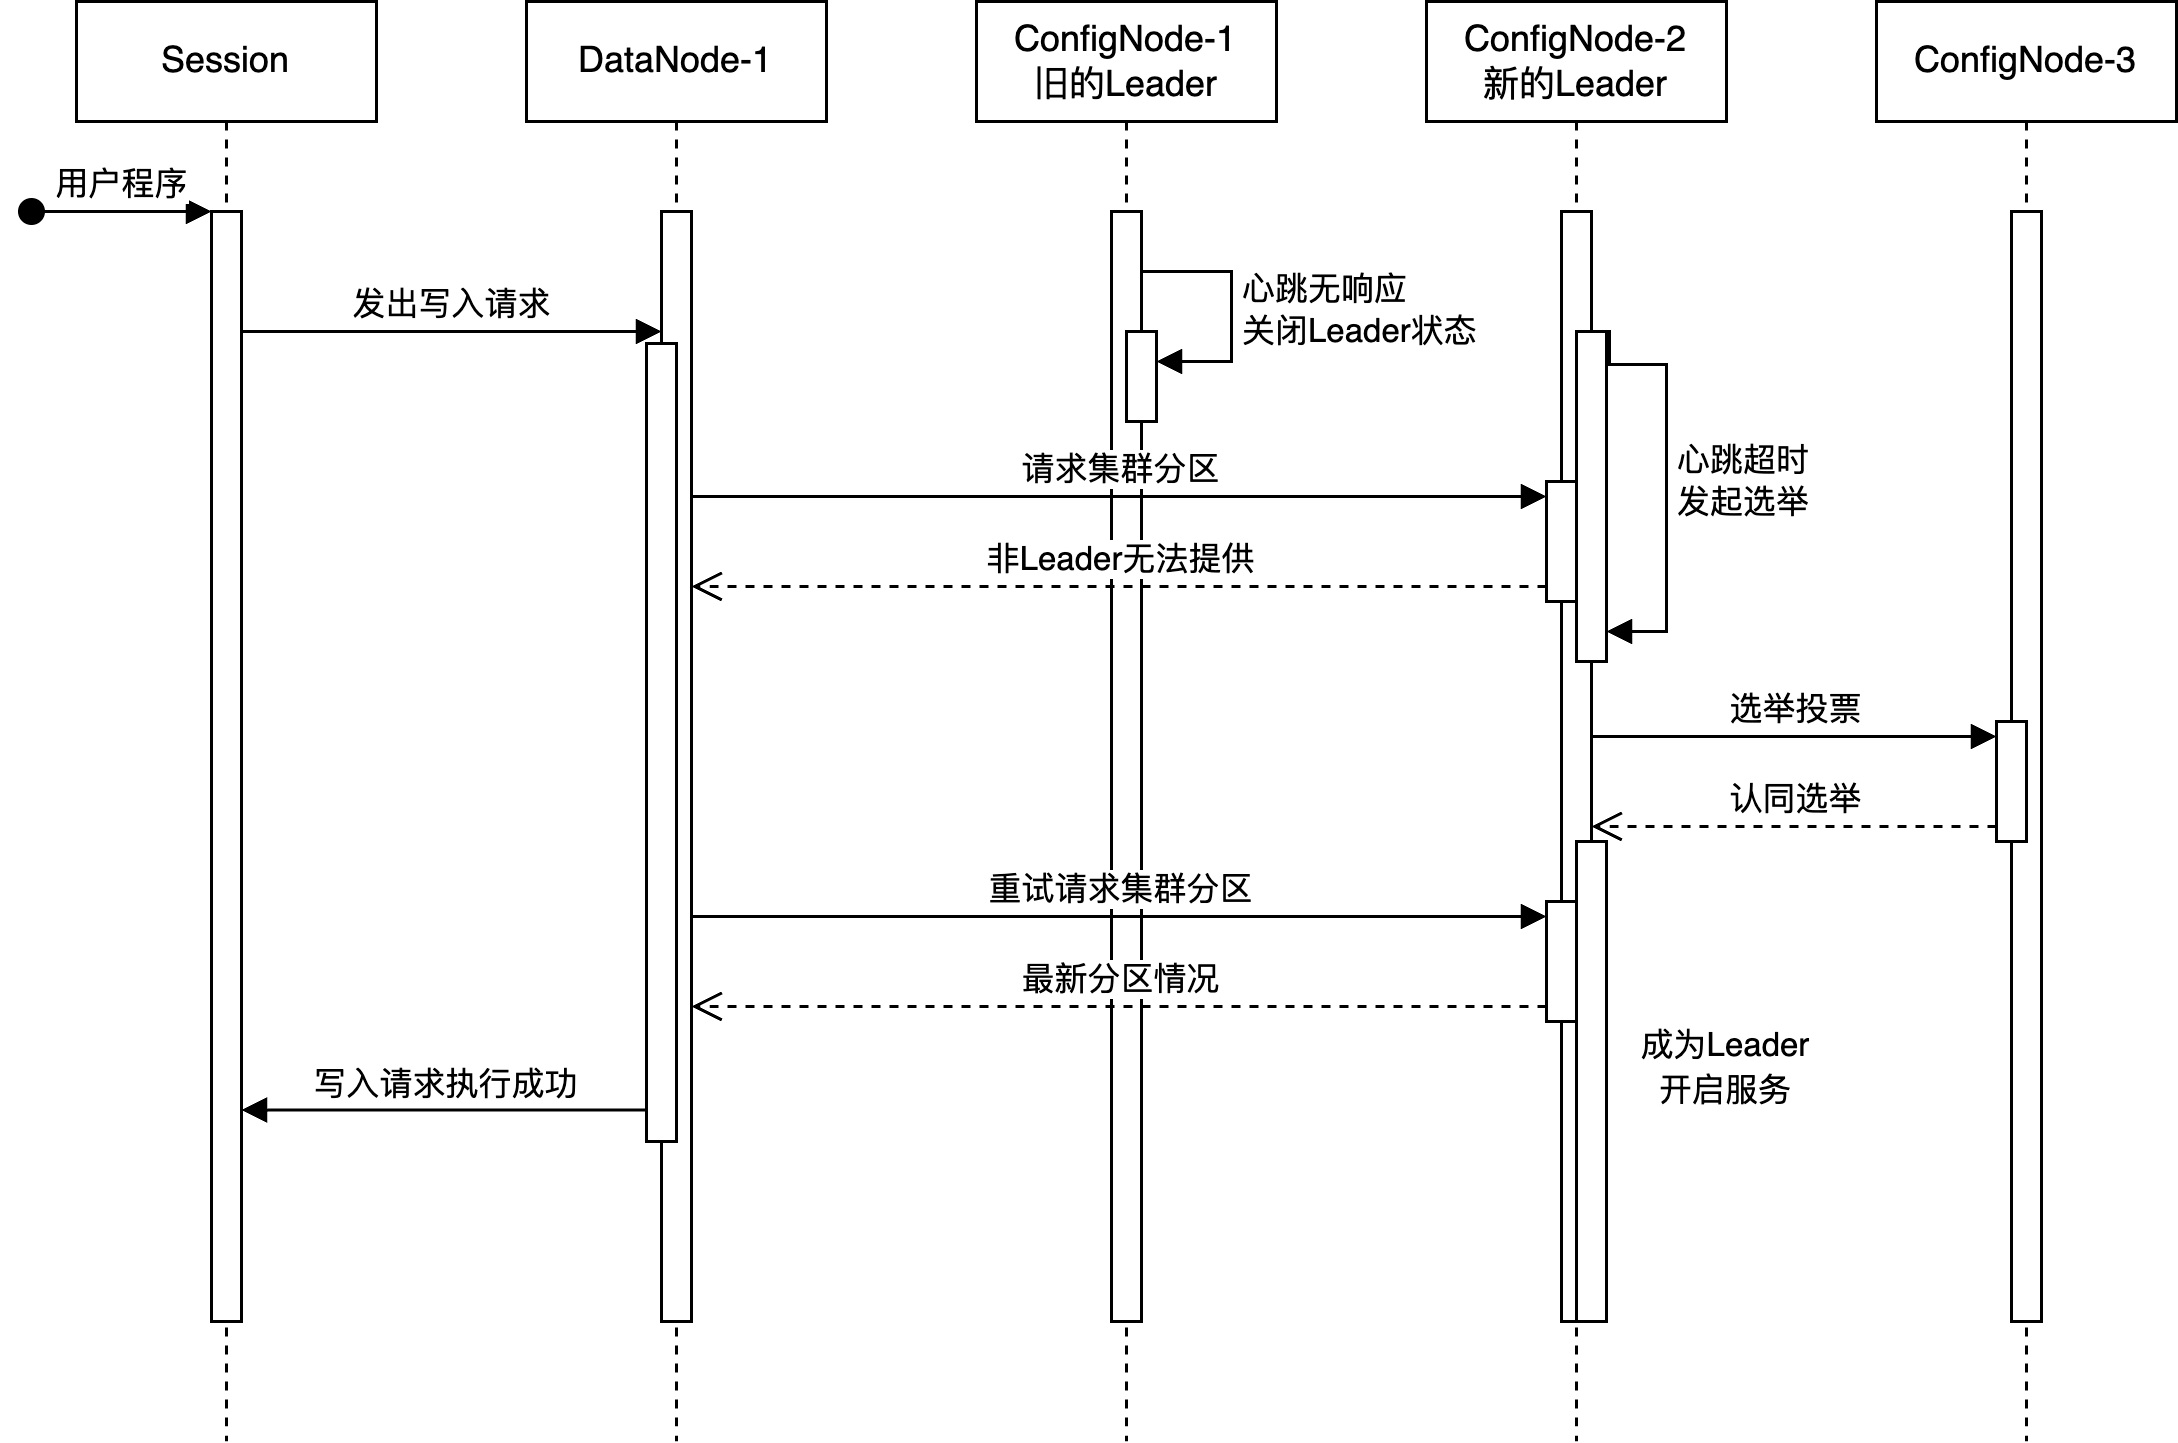
\includegraphics[width=0.99\linewidth]{c05-brain-split.png}
    \caption{ConfigNode服务的高可用容错时序图}
    \label{fig:c05-brain-split}
\end{figure}

图\ref{fig:c05-brain-split}展现了ConfigNode因为短暂的网络分区而导致服务不可用的情况下的高可用时序图。其中,ConfigNode-1是旧的Leader,由于和剩下的两个副本ConfigNode-2/ConfigNode-3之间出现了网络分区,导致在一段时间心跳无响应的状态下失去了租约,主动结束了Leader的服务。此时集群中没有ConfigNode节点能够提供服务。

此时,如果用户的写入和查询请求需要向ConfigNode获取分区等服务,那么这些请求就无法得到响应。比如,DataNode2需要等待一段时间,再进行重试。

在等待的这段时间里,ConfigNode-2率先出现选举超时,开始新一轮的选举,并在ConfigNode3的支持下成功当选最新一期的Leader,并正常开启了ConfigNode 的服务。此时,DataNode2再重试请求分区,ConfigNode2能够正常对其提供服务,DataNode也能够顺利完成请求的执行。


\section{集群变更状态下的一致性}

集群变更状态指的是在Region迁移、扩缩容等场景下,副本会在不同的DataNode之间搬运,集群可能出现短暂的不一致的情况。
例如,Region1的三个副本原先分别在DataNode1、DataNode2、DataNode3上,但是由于新增DataNode4,ConfigNode Leader出于负载均衡的考虑,将DataNode1上的副本迁移向DataNode4。此时,如果写入请求尝试在DataNode1上写入Region1的数据,会导致写入失败,这种失败是由于集群变更的短暂不一致导致的。



\subsection{错误检测}

严格来讲,集群变更的短暂不一致并非故障或错误,而是系统设计的有意为之。

根据CAP原理\cite{fox1999harvest},在一个分布式系统中,一致性(Consistency)、可用性(Availability)、分区容错性(Partition Tolerance)往往无法全部保证。在实际的系统中,分区问题无法避免,因此分区容错性必须保证。这导致了一致性(Consistency)、可用性(Availability)只能二选一。

应用到IoTDB的集群变更场景来说,如果要保证集群变更期间的数据绝对一致性,那么必须暂停所有用户针对变更Region的写入操作,直至变更完成。
这种做法虽然不会让写入和查询请求路由到不存在的影子副本上,但却极大地牺牲了系统的可用性,导致用户在一段时间内无法正常访问或操作数据,这跟本文的理念背道而驰。

因此,IoTDB在设计的时候,选择在保证最终一致性的前提下,允许短暂的数据不一致性。这意味着用户的请求可以随时到达随时执行,即使系统正处在变更的过程中。系统通过Session侧的重试和协调者侧的重试来对数据不一致的问题进行容错。


\subsection{高可用容错方案}

\begin{figure}
    \centering
    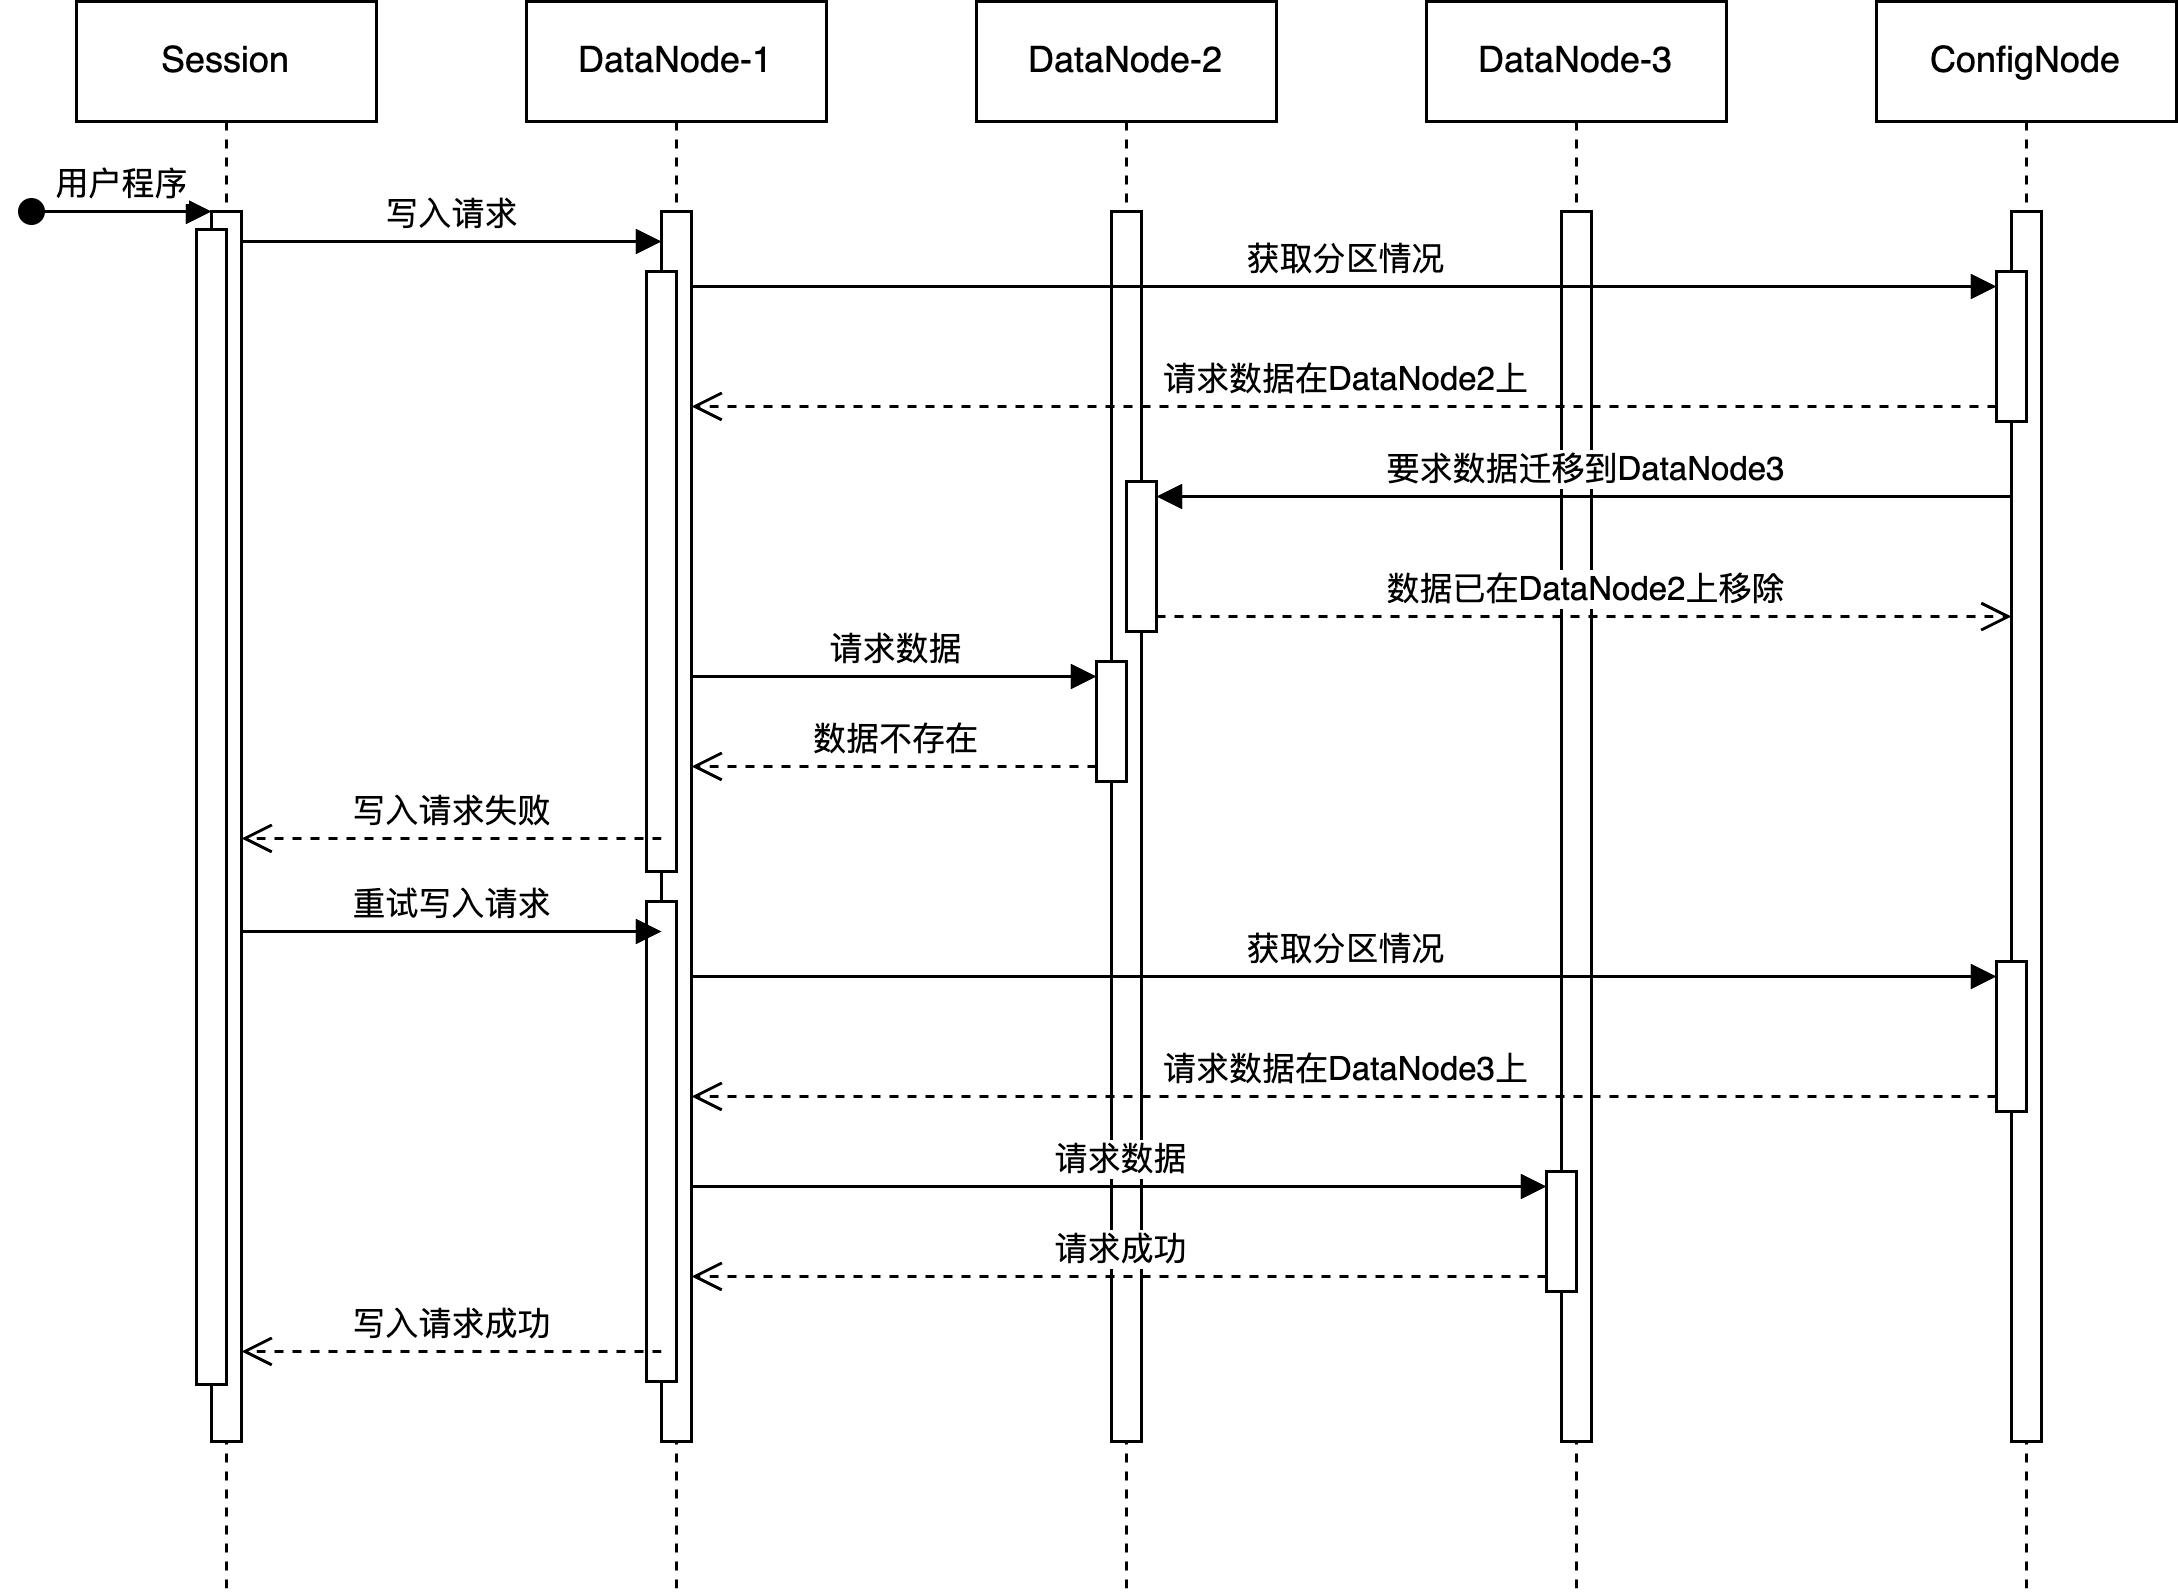
\includegraphics[width=0.99\linewidth]{c05-cluster-change.png}
    \caption{集群变更状态下高可用容错时序图}
    \label{fig:c05-cluster-change}
\end{figure}

图\ref{fig:c05-cluster-change}展示了在集群变更状态下系统的高可用容错时序图。用户在通过Session进行写入请求的时候,DataNode1先从ConfigNode Leader这里获取了分区情况,发现所请求的副本存活在DataNode2上,并根据这个分区情况进行写入规划。
然而在规划完成之后,调度执行之前,处于负载均衡或者扩缩容的考虑,ConfigNode Leader决定进行Region迁移,将原本在DataNode2上的数据副本迁移到DataNode3上。这导致在调度执行的时候,协调者节点依然会向DataNode2上已经不存在的“影子副本”发出请求。
此时,该请求会因为数据不存在而失败,DataNode2会拒绝本次请求,并且附上重试的建议。
如果本Region有多个数据副本,那么协调者节点会首先请求其他的数据副本。在本例中,该Region只有一个副本,因此DataNode1上的协调者节点只能将这次请求失败的信息返回给Session,并且附上重试的建议。
Session会在等待一段时间之后继续重试这个请求。这导致了请求会再次被发送到DataNode1上。此时,DataNode1会再次从ConfigNode这边获取最新的分区情况。此时最新的分区已经能够反映上次迁移的改变,因此DataNode1能够正确认识到数据此时存活在DataNode3上,从而向DataNode3发起请求,最终成功获取数据,本次写入也能顺利执行。
